Physarum presents the intelligence of finding effective solutions to demanding engineering problems such as shortest path problems, various graph problems, evaluation of transport networks or even robotic control.
The most well-known laboratory experiments that the plasmodium of slime mould is subjected to are the imitation and optimization of human-made transport networks and the finding of the shortest path in a maze.
Part of our project is to verify the effective functioning of each model and compare the results obtained simulating the slime mould in predefinite maps.

\par
Our simulations are based on the work of the same research group \cite{dourvas2016gpgpu}, \cite{tsompanas2015cellular} that have reproposed the diffusion equations of the original model \cite{Tsompanas2016} and then have applied those in different contexts.

\par
The model of Tsompanas et al. \cite{Tsompanas2016} has some important alternation from the others cited. In particular, the same diffusion equations are incorporated in an algorithm composed by the following steps:

\begin{enumerate}
	\item Initialize the model: the parameters of the diffusion equations are set and the topology of the SP and the NSs is also introduced
	\item Apply the diffusion equations for 50 time steps
	\item Check if any of the NSs is covered with a predefined percentage of PM (ThPM). If there is at least one NS covered continue, else go to (2).
	\item All NSs covered with the predefined percentage of PM (ThPM), are encapsulated by the plasmodium and therefore connected to a SP.
	\item The NSs mentioned in (4) change into SPs, meaning their PM is set to 100. If no more than 5,000 time steps have passed (t <5,000) go to (2), else continue.
	\item Redefine all the cells of “interest” (NSs and SP) as NSs, except from the second to last NS encapsulated for the previous 5,000 time steps which is redefined as a SP. Execute for a second time (2)–(5) for 5,000 time steps.
\end{enumerate}

Note that some procedures are identical for each work previously analyzed \cite{dourvas2016gpgpu}, \cite{tsompanas2015cellular}. We firstly initialize the parameters, set one SP in the map as the beginning mass value of the plasmodium with a $PM$ value equals to 100 and then in one or more cell we set the NS which has a $CHA$ value equals to 100. Then, an iterative execution of the diffusion equations gives the values of $PM$ and $CHA$ for all the cells in the CA grid.

\par
From here on there are substancial differences in the approaches used. In \cite{dourvas2016gpgpu} and \cite{tsompanas2015cellular} the procedure stops and the algorithm designs the minimum tubular network based on the values of the $PM$ variable. When a cell’s $TE$ = \texttt{true} then the algorithm searches which of its neighbors has the greater value of $PM$. When it finds it, the $TE$ value of neighbor changes from \texttt{false} to \texttt{true}. This procedure is repeated until the final, minimum tube is created between the cell that the plasmodium was first introduced to the cell with the $NS$. 

\par
In \cite{Tsompanas2016}, in addition, there's the last step of the algorithm explained above that is tricky. It redefine all the NSs and SP as NSs, except from the second to last NS encapsulated for the previous 5000 time steps which is redefined as a SP. This happen because as the CA model is designed without the use of probabilistic equations, it uses a second starting point to regenerate and explore the available area once more. That point will be a point of interest (NS), which is empirically chosen to be away from the initial SP. The second to last NS to be encapsulated was chosen, based on the fact that it is far enough from the initial SP and it is less likely to be a point of interest surrounded by unavailable area that would cause difficulties for the growth of the plasmodium. Then this model requests a second time execution of the algorithm steps from 2 to 5 for further 5000 time steps.

\par
This last part of seems to be forcing considering, as we will see in the next sections related to the simulations, that a certain point the computation arrives at a steady state in which the $PM$ covers the map completely with the same value, leading then to a steady state. As mentioned in \cite{dourvas2016gpgpu} usually about a 1700 time steps are required for the CA-modeled plasmodium to explore a $75 \times 75$ map.

\section{Network formation}
In order to evaluate the efficiency of the networks of the bioinspired CA based model, randomly deployed distributions of 20, 40 and 60 nodes are evaluated. The maps are proposed below:

\begin{figure*}
  \centering
    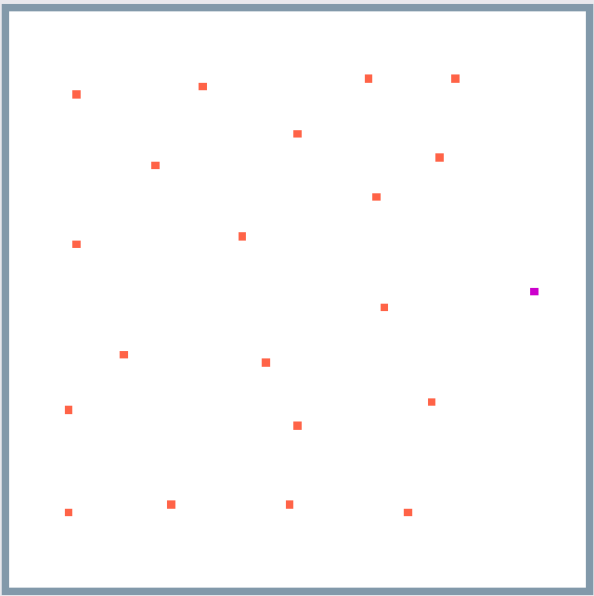
\includegraphics[width=0.8\textwidth]{wsn_20_exp/1_wsn_20}%
    
  \caption{Wsn network with 20 nodes}
  \label{fig:wsn_20_exp/1_wsn_20}
\end{figure*}

\begin{figure*}
  \centering
    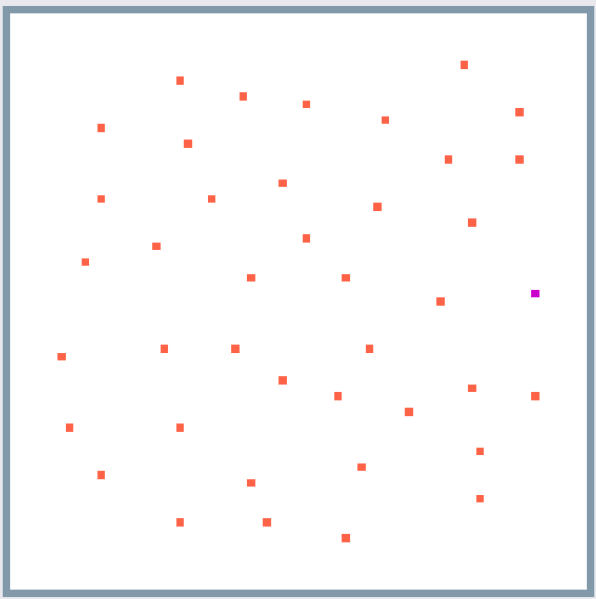
\includegraphics[width=0.8\textwidth]{wsn_40_exp/1_wsn_40}%
    
  \caption{Wsn network with 40 nodes}
  \label{fig:wsn_40_exp/1_wsn_40}
\end{figure*}

\begin{figure*}
  \centering
    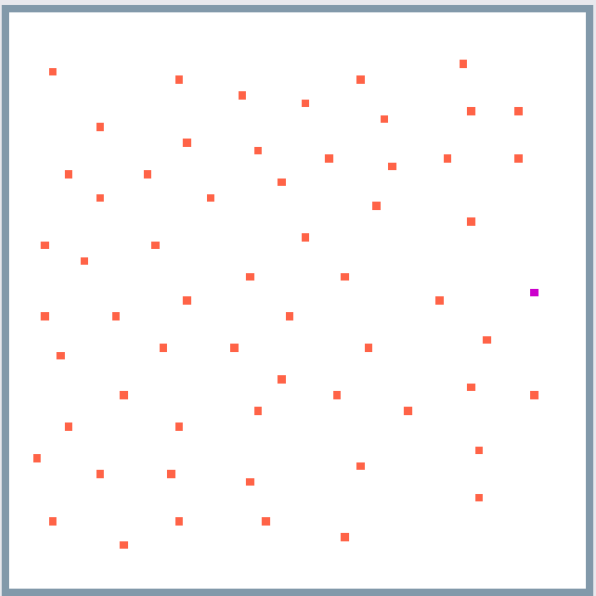
\includegraphics[width=0.8\textwidth]{wsn_60_exp/1_wsn_60}%
    
  \caption{Wsn network with 60 nodes}
  \label{fig:wsn_60_exp/1_wsn_60}
\end{figure*}


These maps are very similar to those proposed in \cite{tsompanas2015cellular} in which the plasmodium of Physarum polycephalum is the inspiration of a CA based model for constructing data trees in a WSN that connect all nodes with a sink node, that is located in the east border of the WSN for each of the three distributions.

\par
The black dot illustrates the location of the sink node and the yellow dots illustrate the locations of the sensing nodes. The topologies of the nodes are used as input for the model, with the sink node represented as the SP and all the other nodes represented as NSs. Furthermore, the initial parameters set for the model are illustrated in the next subsections.

\par
In addition to the previous maps we have also considered as an experiment a network with SP in a centered position, as can be seen in the following figure:

\begin{figure*}
  \centering
    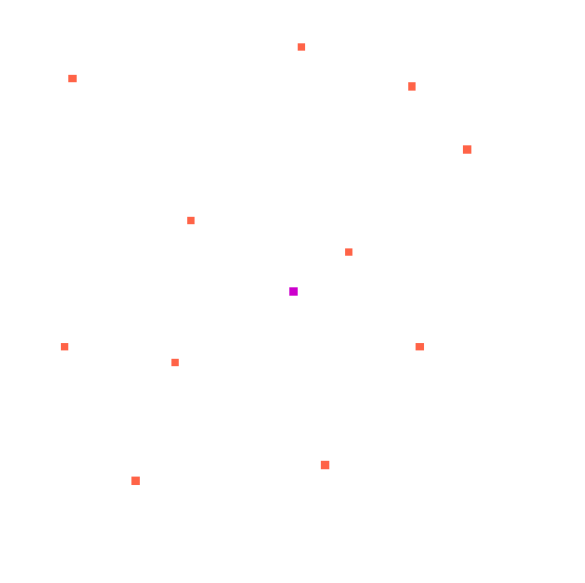
\includegraphics[width=0.8\textwidth]{central_sp_exp/1_central_sp}%
    
  \caption{Network with SP in a centered position}
  \label{fig:central_sp_exp/1_central_sp}
\end{figure*}

\subsection{Paper model}

In this case the parameters are the same for each of the four networks simulated.

\begin{center}
 \begin{tabular}{||c c||} 
 \hline
 Parameter & Value \\ [0.5ex] 
 \hline\hline
 GridSize & $75 \times 75$ \\ 
 \hline
 PM & 100 \\ 
 \hline
 CHA & 100 \\ 
 \hline
 CON & 0.95 \\ 
 \hline
 PAP & 0.8 \\ 
 \hline
 PMP1 & 0.08 \\ 
 \hline
 PMP2 & 0.01 \\ 
 \hline
 CAP1 & 0.05 \\ 
 \hline
 CAP2 & 0.01 \\ 
 \hline
 ThPM & 0.2 \\ [1ex] 
 \hline
 \end{tabular}
\end{center}

Below are shown the simulation for each network. 

\paragraph{Wsn network with 20 NSs}

\begin{figure}[H]
    \centering
    \subfigure[]{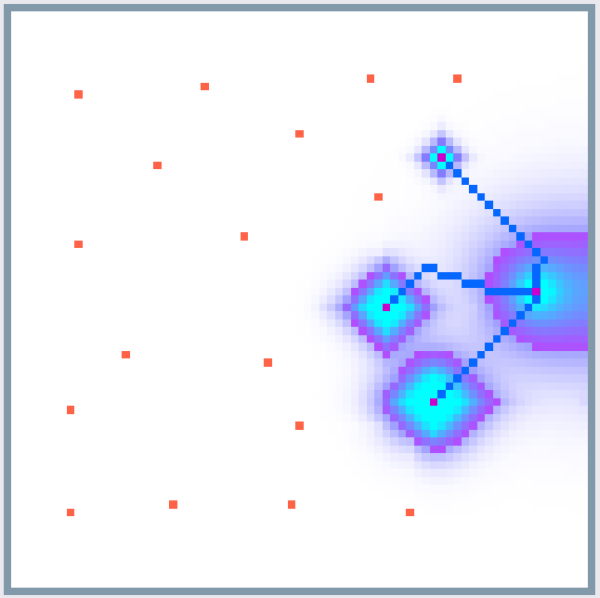
\includegraphics[width=0.40\textwidth]{wsn_20_pap/2_wsn_20}} 
    \subfigure[]{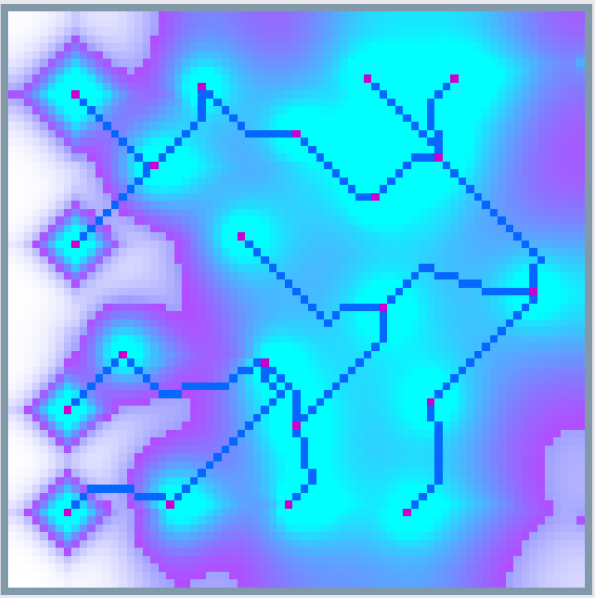
\includegraphics[width=0.40\textwidth]{wsn_20_pap/3_wsn_20}} 
    \caption{(a) Expansion process (b) Simulation end}
    \label{fig:foobar}
\end{figure}

\paragraph{Wsn network with 40 NSs}

\begin{figure}[H]
    \centering
    \subfigure[]{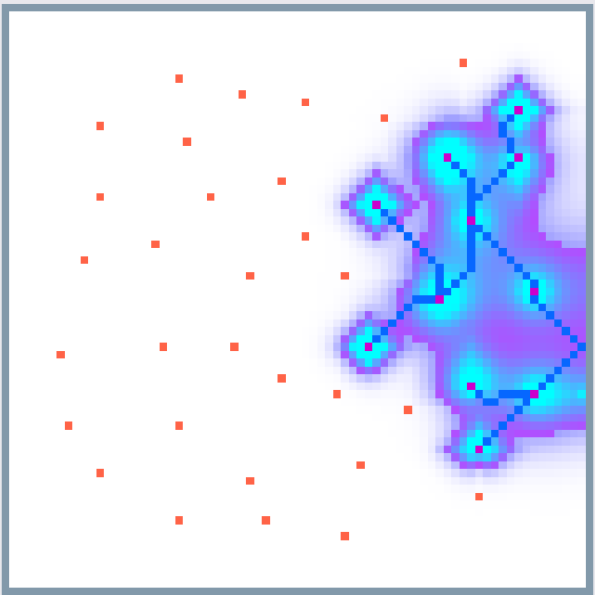
\includegraphics[width=0.40\textwidth]{wsn_40_pap/2_wsn_40}} 
    \subfigure[]{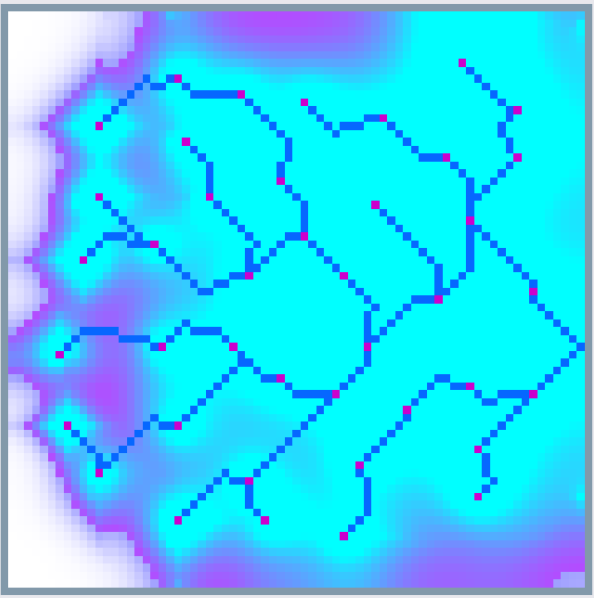
\includegraphics[width=0.40\textwidth]{wsn_40_pap/3_wsn_40}} 
    \caption{(a) Expansion process (b) Simulation end}
    \label{fig:foobar}
\end{figure}

\paragraph{Wsn network with 60 NSs}

\begin{figure}[H]
    \centering
    \subfigure[]{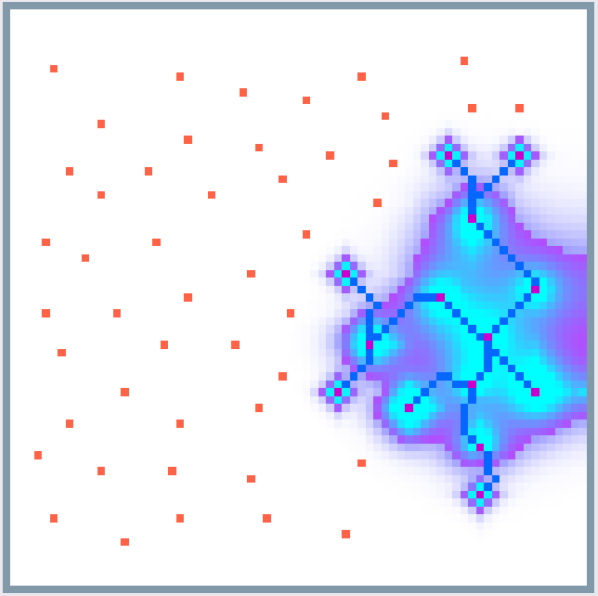
\includegraphics[width=0.40\textwidth]{wsn_60_pap/2_wsn_60}} 
    \subfigure[]{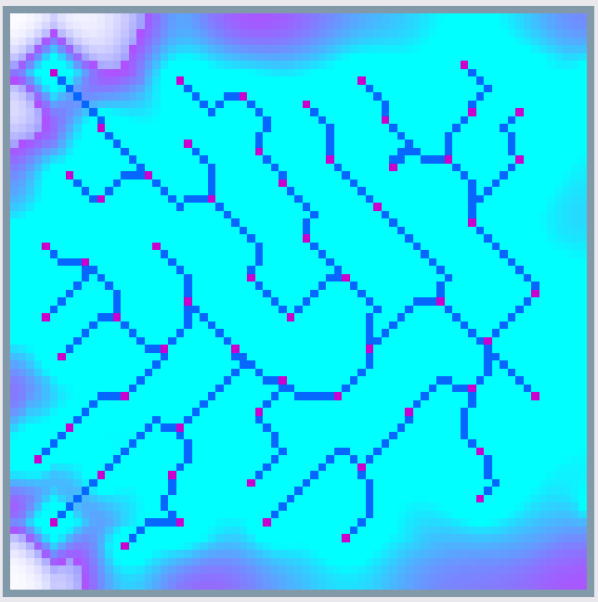
\includegraphics[width=0.40\textwidth]{wsn_60_pap/3_wsn_60}} 
    \caption{(a) Expansion process (b) Simulation end}
    \label{fig:foobar}
\end{figure}

\paragraph{Network with SP in a centered position}
\begin{figure}[H]
    \centering
    \subfigure[]{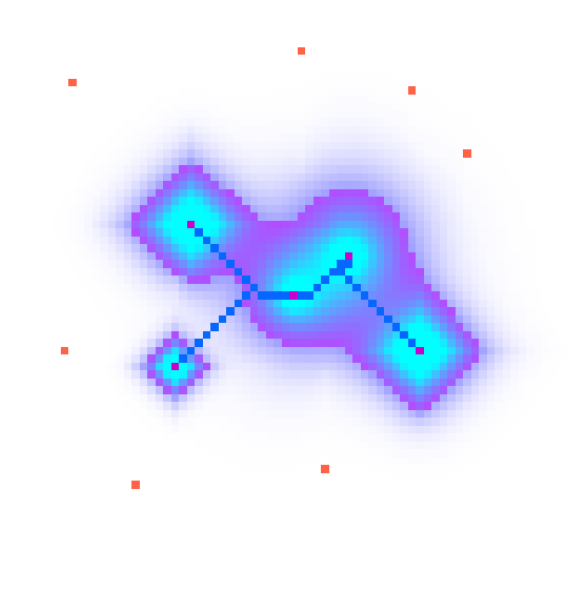
\includegraphics[width=0.40\textwidth]{central_sp_pap/2_central_sp}} 
    \subfigure[]{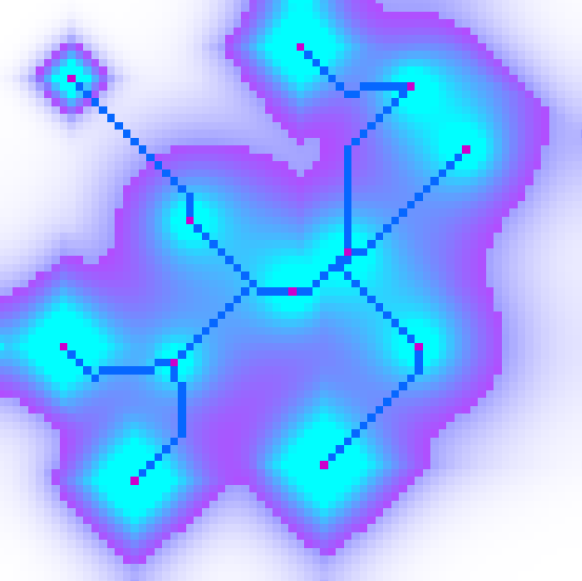
\includegraphics[width=0.40\textwidth]{central_sp_pap/3_central_sp}} 
    \caption{(a) Expansion process (b) Simulation end}
    \label{fig:foobar}
\end{figure}

\subsection{Experimental model}

Also in this case the parameters are the same for each of the four maps simulated.

\begin{center}
 \begin{tabular}{||c c||} 
 \hline
 Parameter & Value \\ [0.5ex] 
 \hline\hline
 GridSize & $75 \times 75$ \\ 
 \hline
 PM & 10000 \\ 
 \hline
 CHA & 100 \\ 
 \hline
 CON & 0.95 \\ 
 \hline
 CAP1 & 0.05 \\ 
 \hline
 CAP2 & 0.01 \\ 
 \hline
 MinAgeDryOut & 1000 \\
 \hline
 ThPM & 20 \\ [1ex] 
 \hline
 \end{tabular}
\end{center}

Below are shown the simulation for each map. 

\paragraph{Wsn network with 20 NSs}

\begin{figure}[H]
    \centering
    \subfigure[]{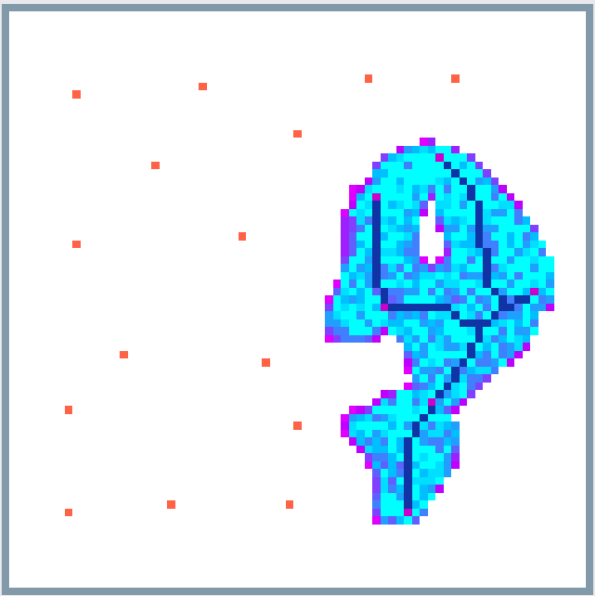
\includegraphics[width=0.32\textwidth]{wsn_20_exp/2_wsn_20}} 
    \subfigure[]{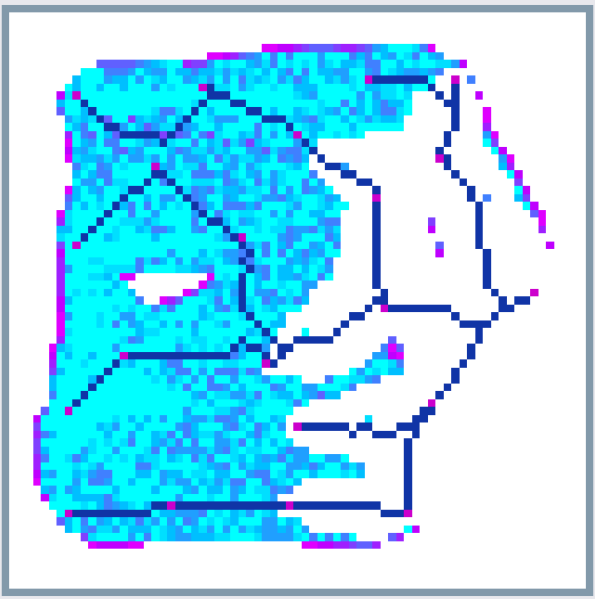
\includegraphics[width=0.32\textwidth]{wsn_20_exp/3_wsn_20}} 
    \subfigure[]{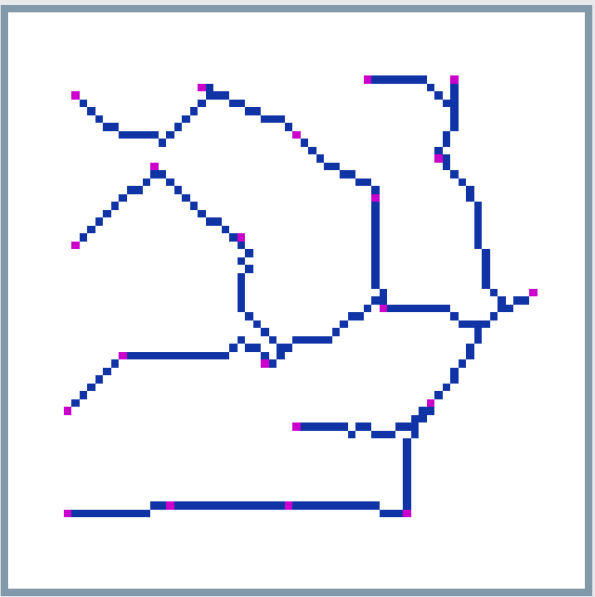
\includegraphics[width=0.32\textwidth]{wsn_20_exp/4_wsn_20}}
    \caption{(a) Expansion process (b) Shrinking process (c) Simulation end}
    \label{fig:foobar}
\end{figure}

\paragraph{Wsn network with 40 NSs}

\begin{figure}[H]
    \centering
    \subfigure[]{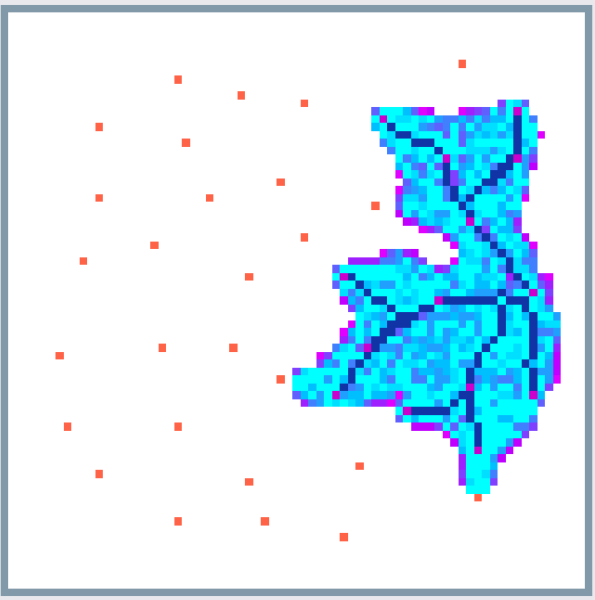
\includegraphics[width=0.32\textwidth]{wsn_40_exp/2_wsn_40}} 
    \subfigure[]{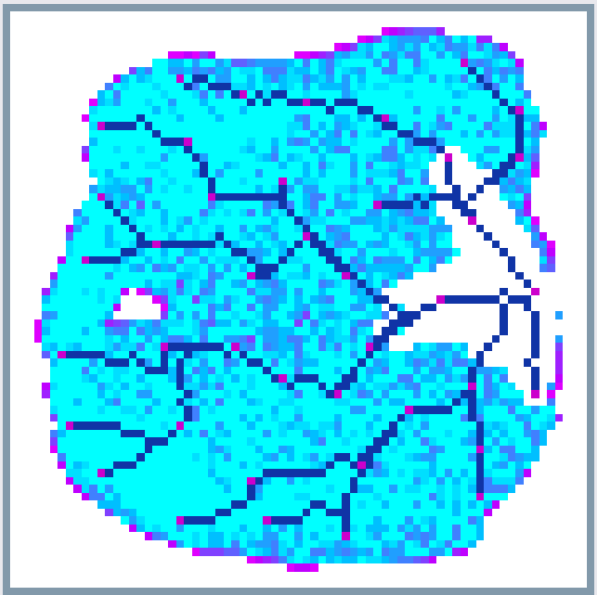
\includegraphics[width=0.32\textwidth]{wsn_40_exp/3_wsn_40}} 
    \subfigure[]{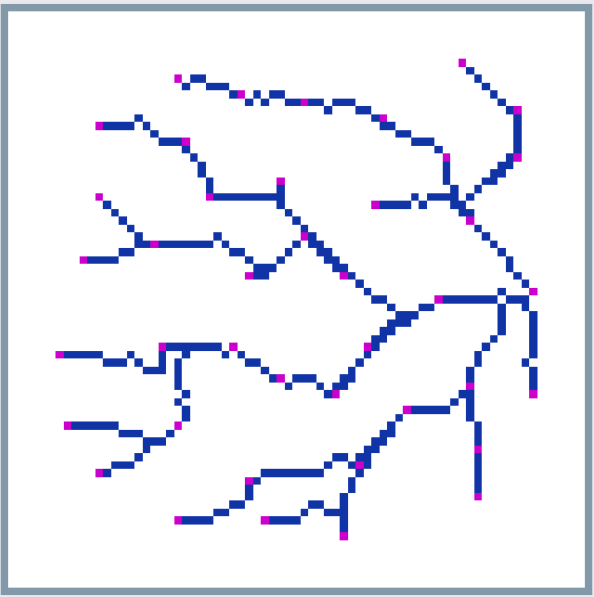
\includegraphics[width=0.32\textwidth]{wsn_40_exp/4_wsn_40}}
    \caption{(a) Expansion process (b) Shrinking process (c) Simulation end}
    \label{fig:foobar}
\end{figure}

\paragraph{Wsn network with 60 NSs}

\begin{figure}[H]
    \centering
    \subfigure[]{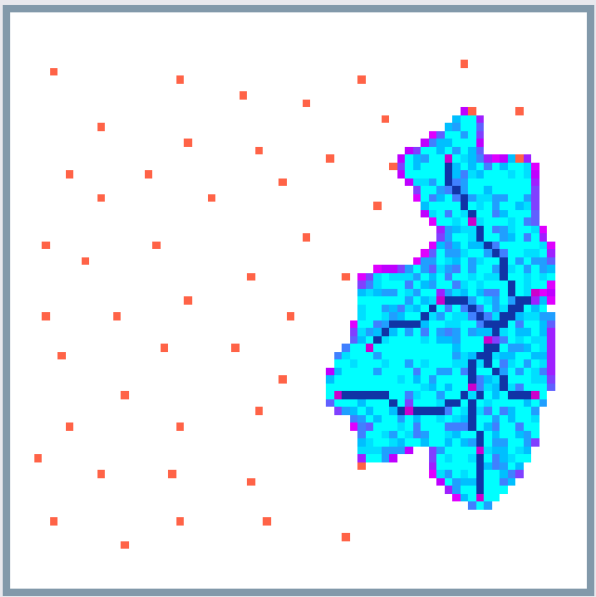
\includegraphics[width=0.32\textwidth]{wsn_60_exp/2_wsn_60}} 
    \subfigure[]{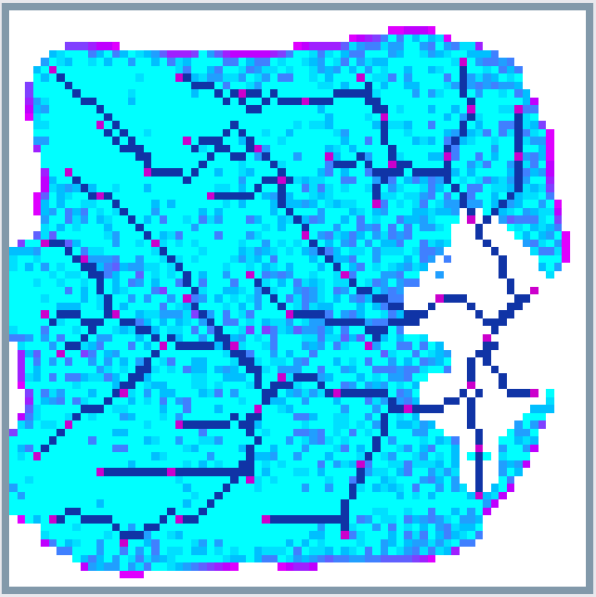
\includegraphics[width=0.32\textwidth]{wsn_60_exp/3_wsn_60}} 
    \subfigure[]{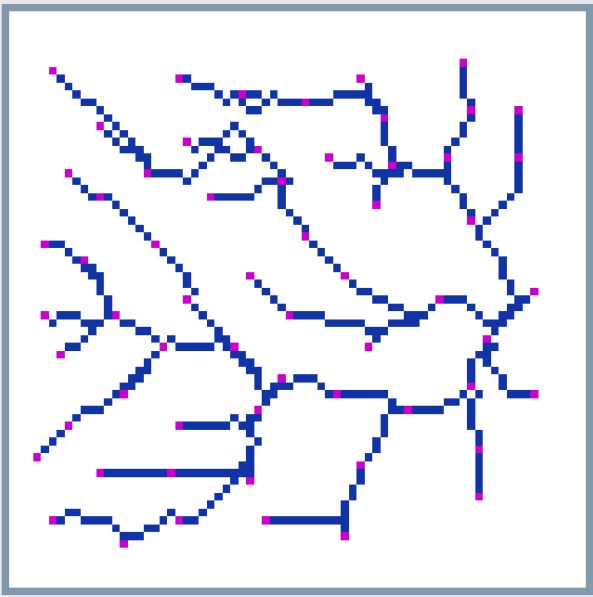
\includegraphics[width=0.32\textwidth]{wsn_60_exp/4_wsn_60}}
    \caption{(a) Expansion process (b) Shrinking process (c) Simulation end}
    \label{fig:foobar}
\end{figure}

\paragraph{Network with SP in a centered position}
\begin{figure}[H]
    \centering
    \subfigure[]{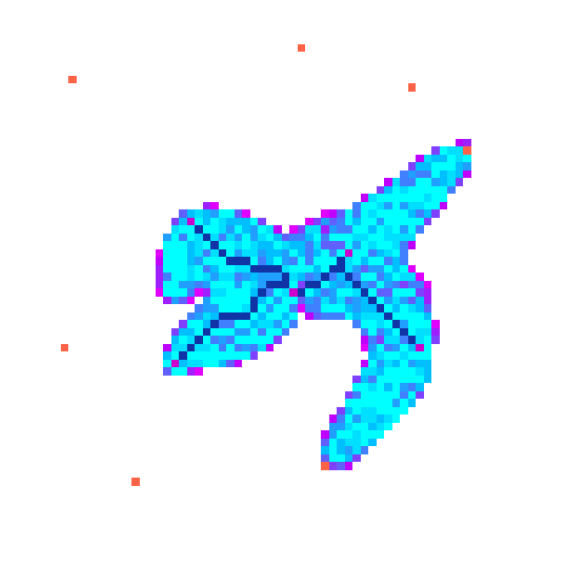
\includegraphics[width=0.32\textwidth]{central_sp_exp/2_central_sp}} 
    \subfigure[]{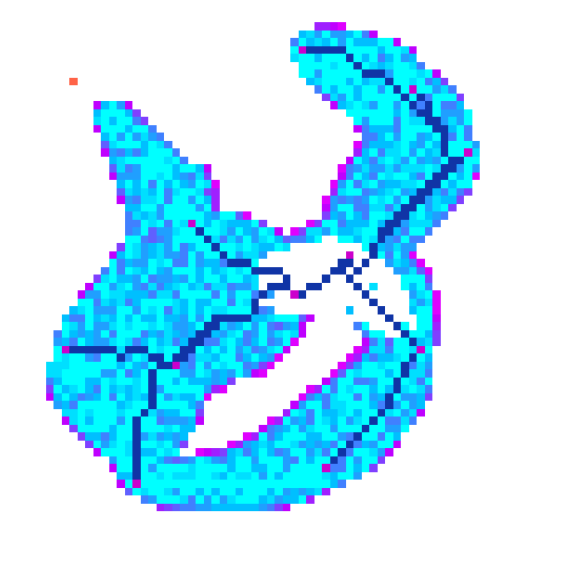
\includegraphics[width=0.32\textwidth]{central_sp_exp/3_central_sp}} 
    \subfigure[]{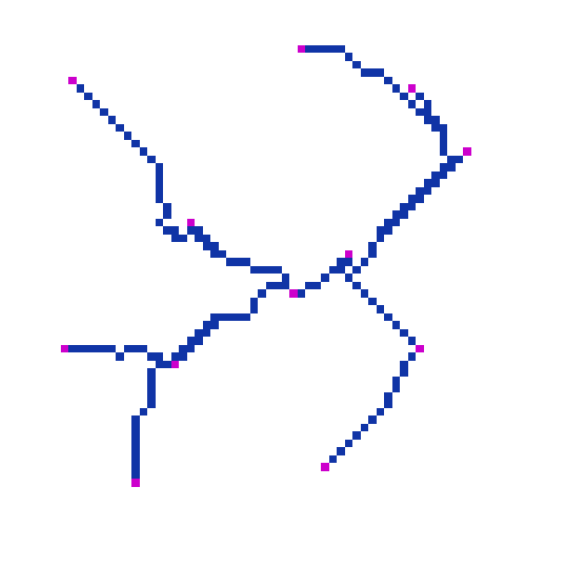
\includegraphics[width=0.32\textwidth]{central_sp_exp/4_central_sp}}
    \caption{(a) Expansion process (b) Shrinking process (c) Simulation end}
    \label{fig:foobar}
\end{figure}

\section{Maze solving}

For the maze solving problem using a Physarum as biological organism two different maps were used: the first maze was faithfully copied from \cite{dourvas2016gpgpu}, while for the second maze we were inspired by one of the most famous experiments \cite{nakagaki2000intelligence} that observed mould behaving like a intelligent organism able to find the minimum-length solution between two points in a maze. The maps in the initial state are proposed below:

\begin{figure*}
  \centering
    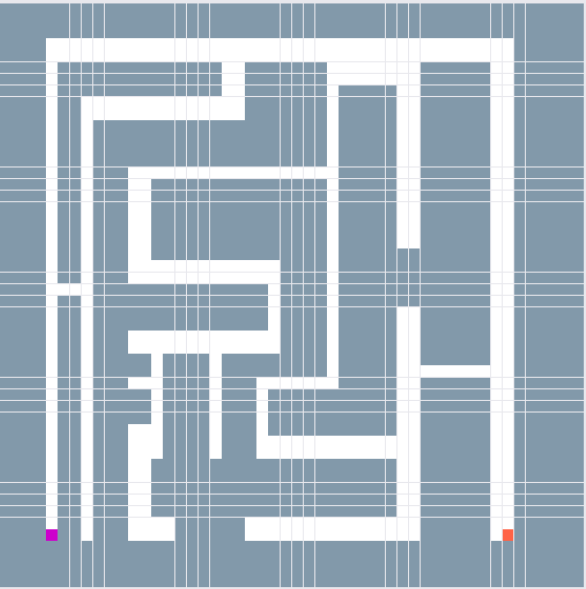
\includegraphics[width=0.8\textwidth]{maze_gpgpu_exp/1_maze_gpgpu}%
    
  \caption{First maze}
  \label{fig:maze_gpgpu_exp/1_maze_gpgpu}
\end{figure*}

\begin{figure*}
  \centering
    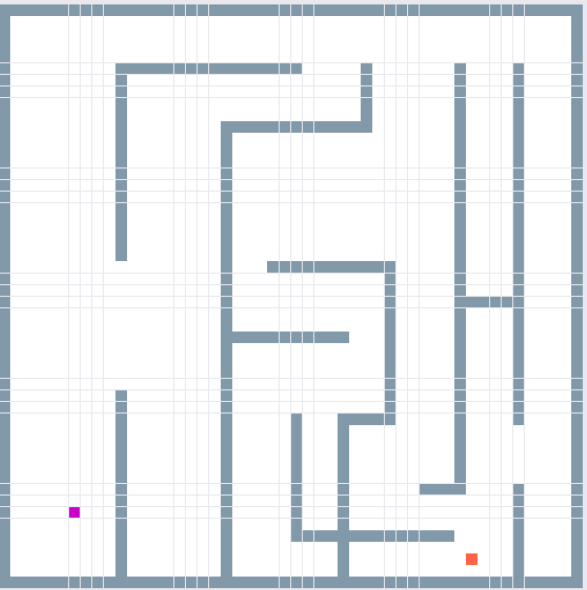
\includegraphics[width=0.8\textwidth]{generic_maze_exp/1_generic_maze}%
    
  \caption{Second maze}
  \label{fig:generic_maze_exp/1_generic_maze}
\end{figure*}

Both maps are presented with an SP and an NS, respectively in the lower left corner and in the lower right corner and then at opposite sides of the maze.

\subsection{Paper model}

For these maps the parameters are different from those applied in the maps representing a network, in particular as regards $PM$ and $CHA$ which are set to 30000 in \cite{dourvas2016gpgpu}.

\begin{center}
 \begin{tabular}{||c c||} 
 \hline
 Parameter & Value \\ [0.5ex] 
 \hline\hline
 GridSize & $50 \times 50$ \\ 
 \hline
 PM & 30000 \\ 
 \hline
 CHA & 30000 \\ 
 \hline
 CON & 0.95 \\ 
 \hline
 CAP1 & 0.05 \\ 
 \hline
 CAP2 & 0.01 \\ 
 \hline
 MinAgeDryOut & 1000 \\
 \hline
 ThPM & 20 \\ [1ex] 
 \hline
 \end{tabular}
\end{center}

\paragraph{First maze}

\begin{figure}[H]
    \centering
    \subfigure[]{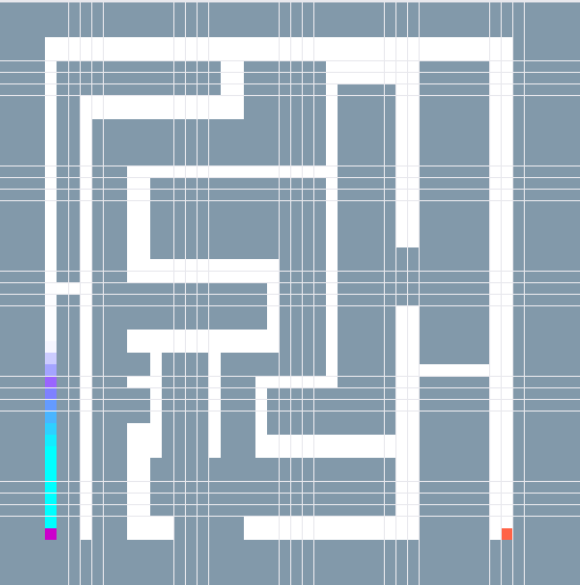
\includegraphics[width=0.40\textwidth]{maze_gpgpu_pap/2_maze_gpgpu}} 
    \subfigure[]{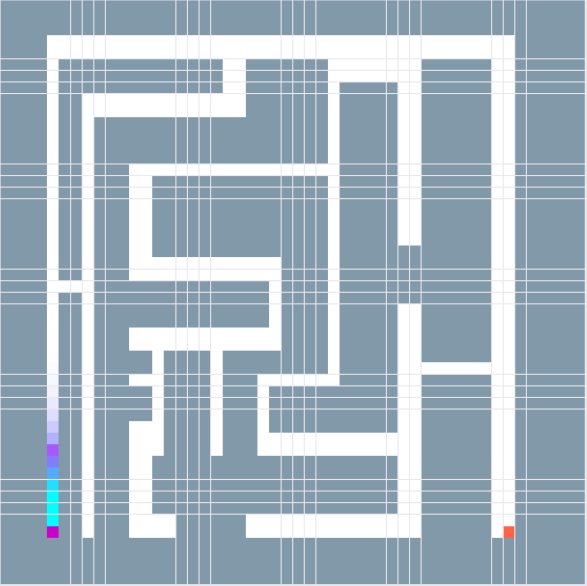
\includegraphics[width=0.40\textwidth]{maze_gpgpu_pap/3_maze_gpgpu}} 
    \caption{(a) Expansion process (b) Last steps}
    \label{fig:foobar}
\end{figure}

In this case the mould stops and begins to regress, failing to complete the maze. The simulation was also made by considerably increasing the initial mass, again achieving poor results.

\paragraph{Second maze}

\begin{figure}[H]
    \centering
    \subfigure[]{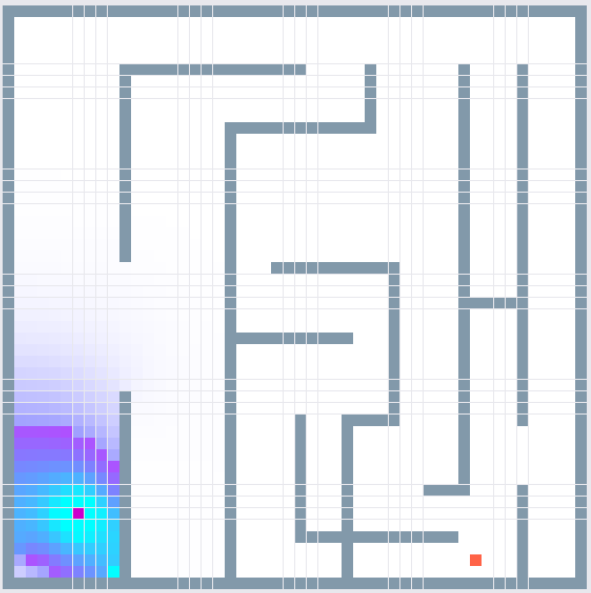
\includegraphics[width=0.40\textwidth]{generic_maze_pap/2_generic_maze}} 
    \subfigure[]{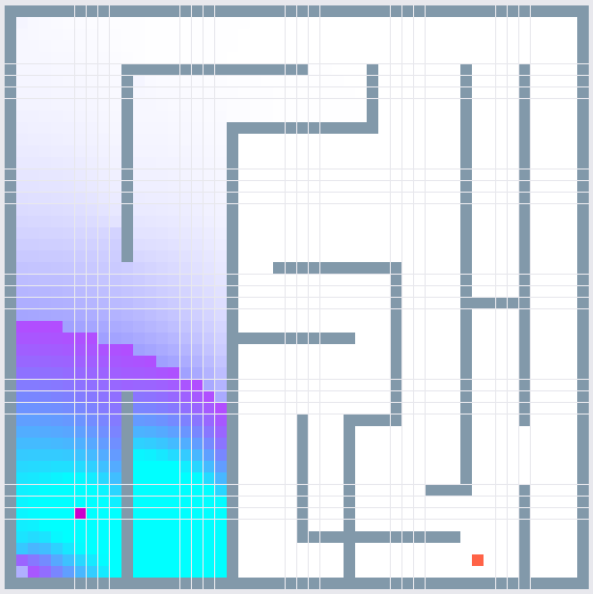
\includegraphics[width=0.40\textwidth]{generic_maze_pap/3_generic_maze}} 
    \caption{(a) Max expansion (b) Regression}
    \label{fig:foobar}
\end{figure}

In this another case the mould after 5050 steps has not yet reached the first NS. There is only one SP but we cannot change it into a NS.

\subsection{Experimental model}

In our model the mould manages to finish the mazes very well in both cases, but with a minimal difference in the MinAgeDryOut variable. Since the distance to be traveled is greater in the first maze, a greater value is needed which has been doubled bringing the value from 1000 of the second maze to 2000. The other values are equivalent for the success of the execution.

\paragraph{First maze}

\subparagraph{Parameters}

\begin{center}
 \begin{tabular}{||c c||} 
 \hline
 Parameter & Value \\ [0.5ex] 
 \hline\hline
 GridSize & $50 \times 50$ \\ 
 \hline
 PM & 10000 \\ 
 \hline
 CHA & 100 \\ 
 \hline
 CON & 0.95 \\ 
 \hline
 CAP1 & 0.05 \\ 
 \hline
 CAP2 & 0.01 \\ 
 \hline
 MinAgeDryOut & 2000 \\
 \hline
 ThPM & 20 \\ [1ex] 
 \hline
 \end{tabular}
\end{center}

\subparagraph{Simulation}

\begin{figure}[H]
    \centering
    \subfigure[]{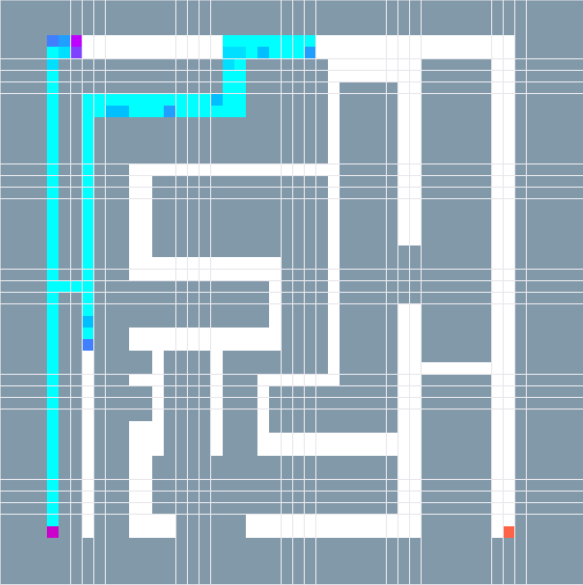
\includegraphics[width=0.32\textwidth]{maze_gpgpu_exp/2_maze_gpgpu}} 
    \subfigure[]{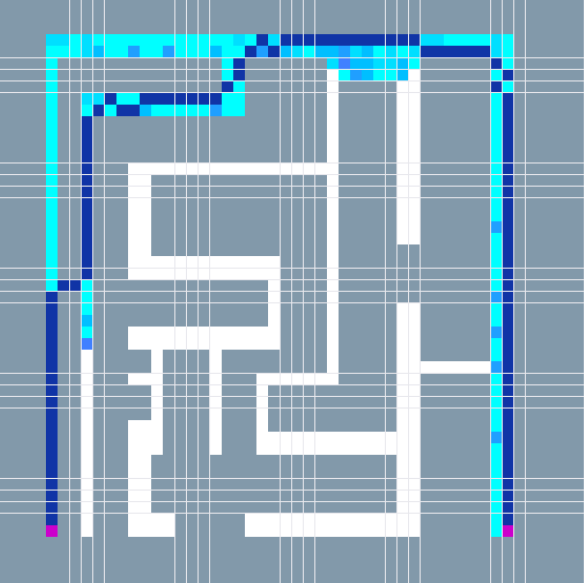
\includegraphics[width=0.32\textwidth]{maze_gpgpu_exp/3_maze_gpgpu}} 
    \subfigure[]{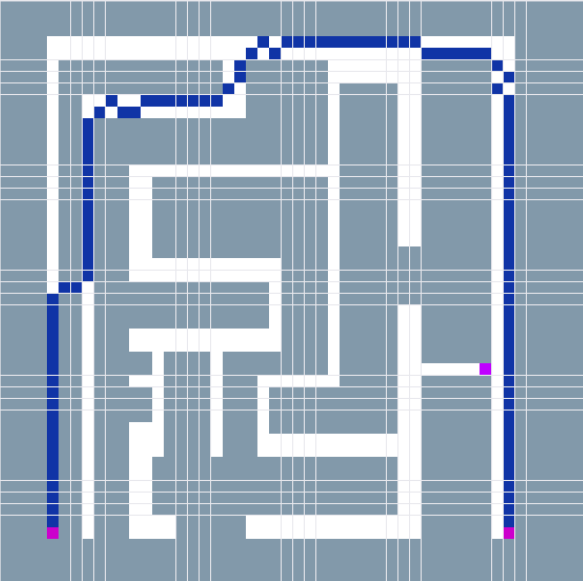
\includegraphics[width=0.32\textwidth]{maze_gpgpu_exp/4_maze_gpgpu}}
    \caption{(a) Expansion process (b) Tubes creation (c) Simulation end}
    \label{fig:foobar}
\end{figure}

\paragraph{Second maze}

\subparagraph{Parameters}

\begin{center}
 \begin{tabular}{||c c||} 
 \hline
 Parameter & Value \\ [0.5ex] 
 \hline\hline
 GridSize & $50 \times 50$ \\ 
 \hline
 PM & 10000 \\ 
 \hline
 CHA & 100 \\ 
 \hline
 CON & 0.95 \\ 
 \hline
 CAP1 & 0.05 \\ 
 \hline
 CAP2 & 0.01 \\ 
 \hline
 MinAgeDryOut & 1000 \\
 \hline
 ThPM & 20 \\ [1ex] 
 \hline
 \end{tabular}
\end{center}

\subparagraph{Simulation}

\begin{figure}[H]
    \centering
    \subfigure[]{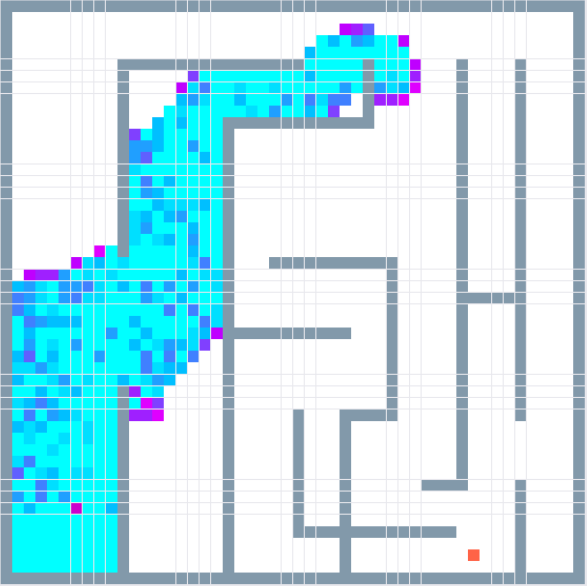
\includegraphics[width=0.32\textwidth]{generic_maze_exp/2_generic_maze}} 
    \subfigure[]{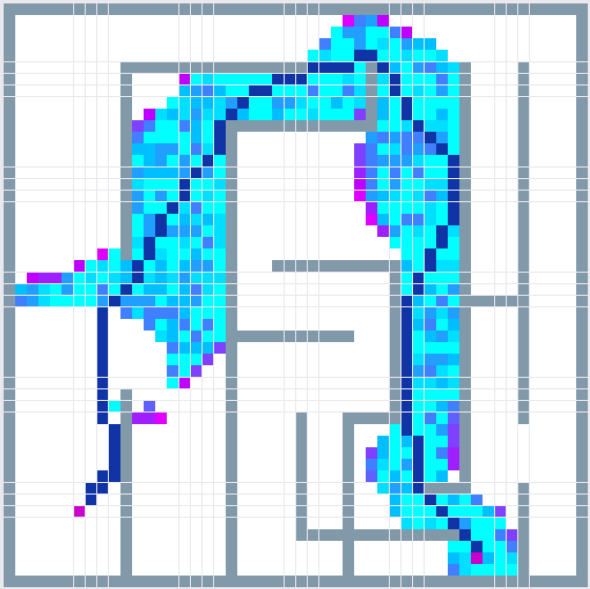
\includegraphics[width=0.32\textwidth]{generic_maze_exp/3_generic_maze}} 
    \subfigure[]{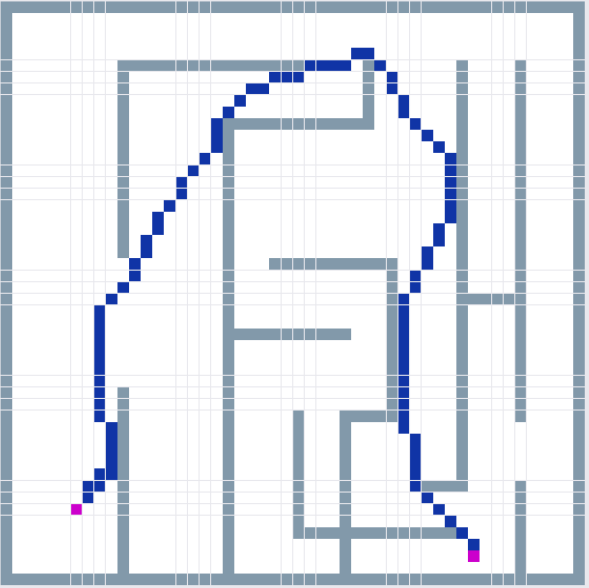
\includegraphics[width=0.32\textwidth]{generic_maze_exp/4_generic_maze}}
    \caption{(a) Expansion process (b) Tubes creation and shrinking process (c) Simulation end}
    \label{fig:foobar}
\end{figure}
